\chapter{System description}\label{se:system_description}
This section will go into details of the structure of the sewer network for which the further work of this project will be based upon.

As mentioned in section \ref{se:chemical_process} a steady flow of sewage with a fixed level of contaminants is desired such that an optimal utilization of the wastewater treatment plant can be obtained. An area of interest is Fredericia with a sizable population of approximately 40.000 people and industries where some of the largest consists of a brewery, bottling plant, refinery and a dairy plant \cite{Statistic_Denmark}. All of these industries is placed in the outskirts of the city, meaning that the wastewater discharged into the sewer goes through populated areas creating an uneven flow of sewage to the wastewater treatment plant. Two main sewer lines separates the northern and southern part of the city. To limit the project only the northern main sewer line is considered, which covers the largest part of the households and the industry located in the city. % This excludes the dairy from the scope of the project as it is located southeast from the wastewater treatment plant. 
In figure \ref{fig:kloakgrid_simplified} a simplified overview of the northern main sewer line with the various areas of population and industry in Fredericia attached to it. The placement of the sewers shown in \ref{fig:kloakgrid_simplified} is obtained from a Geographically Information System (GIS) map publicly available by the municipal of Fredericia \cite{GIS_kort}. The red and the green lines indicate sewers with flows of wastewater and combined wastewater and surface runoff respectively. The populated areas are indicated by two different transparent blue colors, for easier to distinguish between the different parts of the sewer network. The red transparent areas indicate small to medium sized industry. 
Only the sewer lines out of or between the separate areas are shown. Furthermore the areas connected by a red line has a separate sewer system for surface runoff, which is lead into various ponds or the sea, minimizing the load on the wastewater treatment plant.
The bottling plant, refinery and the brewery is marked by the purple, brown and black rings respectively. Several inlets for surface runoff connected directly to the main sewer line exists. The added disturbance from these inlets is neglected on the assumption that the disturbances from the connected areas will be considerable larger.  



\begin{figure}[H]
\centering
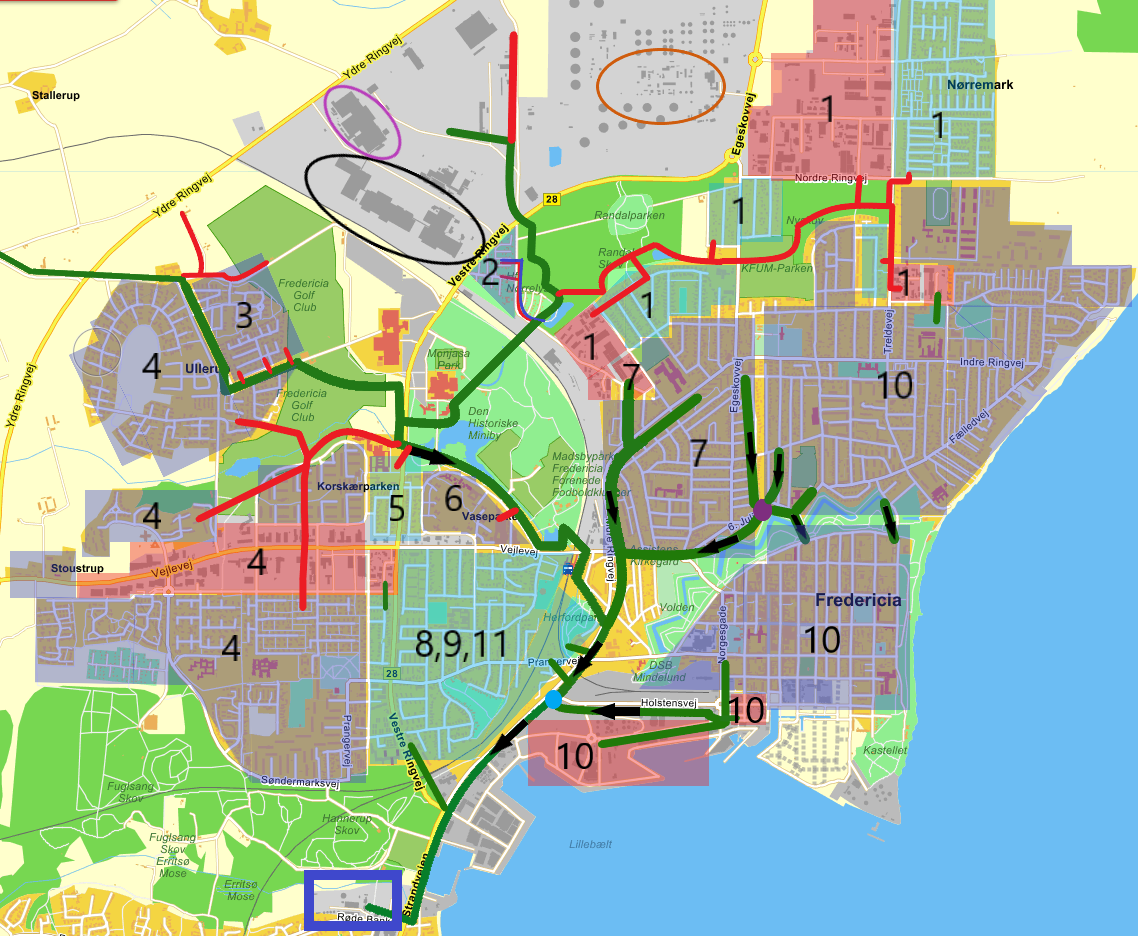
\includegraphics[width=1\textwidth]{report/system_overview/pictures/kloakgrid_simplified8.png}
\caption{Simplified mapping of the northern part of the sewer network in Fredericia. The two blue transparent colors indicate populated areas and the red transparent area indicate industry. Red and green lines is sewers with flows of wastewater and combined wastewater and surface runoff  respectively. Bottling plant, refinery and brewery is marked by purple, brown and black circles respectively. The purple dot is a connecting point with two incoming and two outgoing sewer lines. Blue dot is a wastewater reservoir. Blue rectangle marks the location of the wastewater treatment plant.
%Mapping of part of the sewer network in Fredericia. The red and green lines indicate sewers where the red sewers has flows of sewage only and the green line is combined sewage and runoff from urban surfaces. Transparent parts indicate that the area has a connected sewer grid within and the red/green lines from this grid indicates the output from this area. Two shades of transparent blue is used to illustrate sewer systems in populated areas. The red transparent areas indicate minor industry and the black, brown and purple rings is brewery, refinery and bottling plant respectively. The purple dot indicate a splitting point with two incoming and outgoing sewer pipes. The light blue dot is a sewer reservoir before wastewater is led to the wastewater treatment plant indicated by the blue rectangle.
\cite{Krak}}
\label{fig:kloakgrid_simplified}
\end{figure}
\fxnote{(The blue dot is a sewer reservoir)this is a guess pt. so might need to be corrected}

The various enumerated parts in figure \ref{fig:kloakgrid_simplified} is shown by order of attachment to the main sewer line, together with distance between each attachment, in figure \ref{fig:sewer_line_diagram}. 

\begin{figure}[H]
\centering
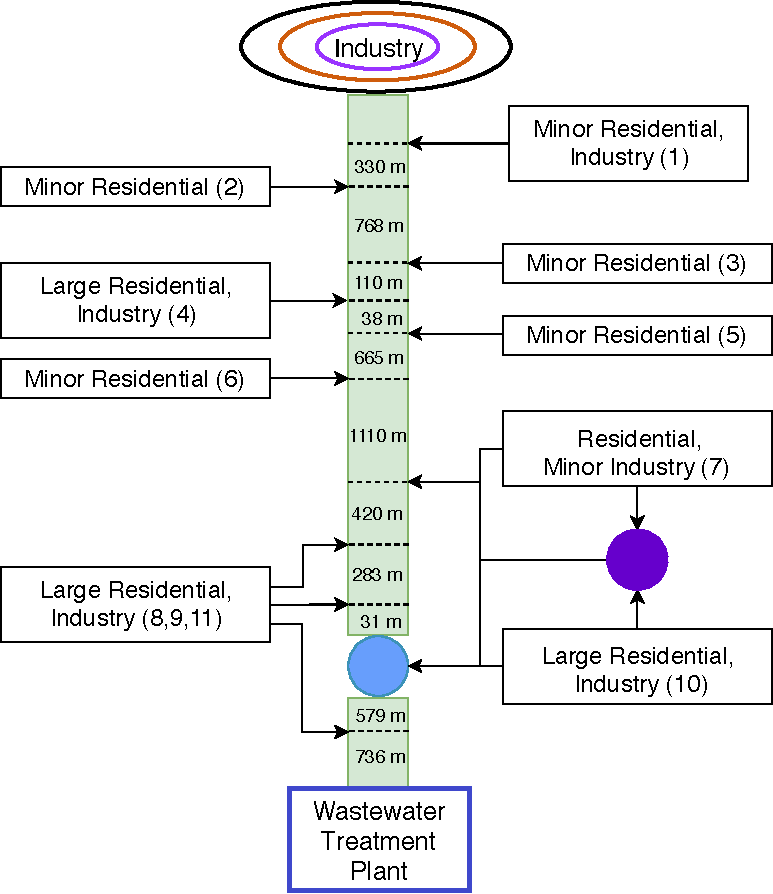
\includegraphics[width=0.6 \textwidth]{report/system_overview/pictures/sewer_line_diagram.pdf}
\caption{Simplification of the attachments to the main sewer line shown in figure \ref{fig:kloakgrid_simplified}. The numbers correspond to which area is connected to the main sewer line farthest from the wastewater treatment plant, with the distance between them.}
\label{fig:sewer_line_diagram}
\end{figure}

Furthermore the different sections consist of pipe of varying diameters as can be seen in table \ref{tab:kloak_diameter}.

% \begin{table} 
% \centering
% \begin{tabular}[H]{|c|c|c|} \hline
% %\begin{table}[H]

% \multirow{2}{*}{Pipe section} & Pipe length & Inner pipe diameter \\ 
% 							  & (meter)		& (millimeter)		\\ \hline
% \multirow{2}{*}{1 $\rightarrow$ 2}		  & 303			  & 900	\\
% 						 & 27			  & 1000 \\ \hline
% 						 & 155			  & 1000 \\
% 2 $\rightarrow$ 3		 & 295			  & 800  \\
% 			 			 & 318			  & 900 \\ \hline
% 3 $\rightarrow$ 4		 & 110			  & 900 \\ \hline
% 4 $\rightarrow$ 5		 & 38 			  & 1000 \\ \hline
% 5 $\rightarrow$ 6		 & 665			  & 1000 \\ \hline
% \multirow{2}{*}{6 $\rightarrow$ 7}		 & 155			  & 1000 \\
% 			 			 & 955			  & 1200 \\ \hline
%  						 & 293			  & 1200 \\
% 7 $\rightarrow$ 8		 & 11 			  & 1300 \\
% 			 			 & 116			  & 1200 \\ \hline
% 8 $\rightarrow$ 9		 & 283			  & 1400 \\ \hline
% 9 $\rightarrow$ 10		 & 31			  & 1400 \\ \hline
% 						 & 125			  & 1600 \\
% 10 $\rightarrow$ 11	 	 & 94			  & 1500 \\
% 						 & 360 			  & 1600 \\ \hline
% 11 $\rightarrow$ WWTP    & 736			  & 1600 \\ \hline
% Total length 		     & \multirow{2}{*}{5070}  &		 \\ 
% 1 $\rightarrow$ WWTP     &						  & \\ \hline

% \end{tabular}

% \caption{Table of the various lengths and the approximate inner diameter of pipe, appearing in order, in the main sewer line. Pipe section indicate the length of pipe between the attachment of the various areas to the main sewer line.} 
% \label{tab:kloak_diameter}
% \end{table}


\begin{table} [H]
\centering
\begin{tabular}{|c|c|c|} 
\hline
\rowcolor[HTML]{9B9B9B} 
\multicolumn{1}{|c|}{\cellcolor[HTML]{9B9B9B}\textbf{Pipe section}} & \multicolumn{1}{c|}{\cellcolor[HTML]{9B9B9B}\textbf{\begin{tabular}[c]{@{}c@{}}Pipe length\\ (meter)\end{tabular}}} & \multicolumn{1}{c|}{\cellcolor[HTML]{9B9B9B}\textbf{\begin{tabular}[c]{@{}c@{}}Inner pipe diameter\\ (millimeter)\end{tabular}}} \\ \hline
\multirow{2}{*}{1 $\rightarrow$ 2}		  & 303			  & 900	\\
						 & 27			  & 1000 \\ \hline
						 & 155			  & 1000 \\
2 $\rightarrow$ 3		 & 295			  & 800  \\
			 			 & 318			  & 900 \\ \hline
3 $\rightarrow$ 4		 & 110			  & 900 \\ \hline
4 $\rightarrow$ 5		 & 38 			  & 1000 \\ \hline
5 $\rightarrow$ 6		 & 665			  & 1000 \\ \hline
\multirow{2}{*}{6 $\rightarrow$ 7}		 & 155			  & 1000 \\
			 			 & 955			  & 1200 \\ \hline
 						 & 293			  & 1200 \\
7 $\rightarrow$ 8		 & 11 			  & 1300 \\
			 			 & 116			  & 1200 \\ \hline
8 $\rightarrow$ 9		 & 283			  & 1400 \\ \hline
9 $\rightarrow$ 10		 & 31			  & 1400 \\ \hline
						 & 125			  & 1600 \\
10 $\rightarrow$ 11	 	 & 94			  & 1500 \\
						 & 360 			  & 1600 \\ \hline
11 $\rightarrow$ WWTP    & 736			  & 1600 \\ \hline
Total length 		     & \multirow{2}{*}{5070}  &		 \\ 
1 $\rightarrow$ WWTP     &						  & \\ \hline

\end{tabular}

\caption{Table of the various lengths and the approximate inner diameter of pipe, appearing in order, in the main sewer line. Pipe section indicate the length of pipe between the attachment of the various areas to the main sewer line.} 
\label{tab:kloak_diameter}
\end{table}